\begin{enumerate}
  \item Sea $W(i,r)$ el peso mínimo para alcanzar, eligiendo entre los primeros $i$ elementos, un valor de al menos $r$, para $i \in \{0,\ldots,n\}$, $r \in \{0,\ldots,V\}$. Es decir, $r$ representa cuánto valor \emph{falta todavía} por conseguir ($r=0$ significa que el requisito ya se cumplió).

  \[
  W(i,r) =
  \begin{cases}
  0 & \text{si } r = 0 \\
  \infty & \text{si } r > 0 \text{ y } i = 0 \\
  \min\big(W(i-1,r),\ \text{weight}[i] + W(i-1,\ \max(0,\, r-\text{value}[i]))\big) & \text{si } r > 0 \text{ y } i > 0
  \end{cases}
  \]

  La respuesta al problema es $W(n,V)$.

  \begin{itemize}
    \item $W(i,r)$: peso mínimo para completar, usando entre los primeros $i$ elementos, un valor acumulado de al menos $r$.
    \item $i$: cuántos de los $n$ elementos candidatos (en el orden en que se listan) se están considerando todavía.
    \item $r$: cuánto valor falta todavía por alcanzar del requisito total $V$.
    \item El $\min$: entre no tomar el elemento $i$ ($W(i-1,r)$, sigue faltando el mismo valor $r$) y tomarlo (se paga $\text{weight}[i]$ y el valor que falta baja a $\max(0, r-\text{value}[i])$, nunca por debajo de $0$), se toma la que resulte en menos peso. Siempre es válido tomar el elemento $i$: no hay condición de ``no cabe'', porque no hay límite de peso, solo se paga su costo.
  \end{itemize}

  \pagebreak

  \item Una tabulación de $W$ tiene complejidad espacial $\Theta(nV)$: una entrada por cada combinación de $i$ y $r$. Pero $W(i,\cdot)$ solo depende de $W(i-1,\cdot)$ (nunca de capas anteriores ni de la misma), así que el grafo de dependencias es por capas, una por cada $i$:

\begin{center}
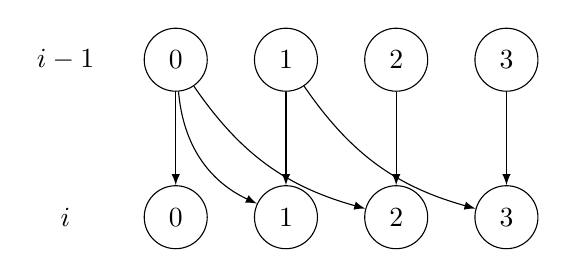
\begin{tikzpicture}[
  vertex/.style={circle, draw, minimum size=0.8cm, inner sep=0pt},
  -latex,
]
  \foreach \r in {0,...,3} {
    \node[vertex] (a\r) at (1.4*\r, 0) {\r};
    \node[vertex] (b\r) at (1.4*\r, -2) {\r};
  }
  \node at (-1.4, 0) {$i-1$};
  \node at (-1.4, -2) {$i$};

  \draw (a0) to (b0);
  \draw (a1) to (b1);
  \draw (a2) to (b2);
  \draw (a3) to (b3);

  % value[i] = 2, así r - value[i] se capa en 0 para r=1,2
  \draw (a0) to[bend right=20] (b2);
  \draw (a0) to[bend right=30] (b1);
  \draw (a1) to[bend right=20] (b3);
\end{tikzpicture}

Dependencias de la capa $i$ hacia la capa $i-1$, para $\text{value}[i]=2$ y $V=3$: cada $(i,r)$ depende de $(i-1,r)$ (no tomar el elemento) y de $(i-1,\max(0,r-\text{value}[i]))$ (tomarlo). Nótese que $r=1$ y $r=2$ ambos apuntan a $(i-1,0)$ al tomarlo, porque el valor sobrante se capa en $0$.
\end{center}

  Como cada capa solo depende de la inmediatamente anterior, no hace falta conservar la tabla completa: basta un arreglo de tamaño $V+1$ actualizado capa por capa, siempre que $r$ se recorra en orden \emph{decreciente} dentro de cada capa (así $W(i-1,\max(0,r-\text{value}[i]))$ no ha sido sobreescrito todavía cuando se necesita, pues $\max(0,r-\text{value}[i]) \le r$). Esto reduce el espacio a $\Theta(V)$, sin cambiar el tiempo: cada uno de los $\Theta(nV)$ estados se resuelve con trabajo $\Theta(1)$, así que la complejidad temporal es $\Theta(nV)$.

  \pagebreak

  \item Tabulación bottom-up en Python, con el arreglo de una sola capa (espacio $\Theta(V)$, tiempo $\Theta(nV)$):

\begin{pseudocode}
def peso_minimo(weight: list[int], value: list[int], V: int) -> int:
    n = len(weight)
    W = [float('inf')] * (V + 1)
    W[0] = 0

    for i in range(n):
        for r in range(V, 0, -1):
            r_restante = max(0, r - value[i])
            W[r] = min(W[r], weight[i] + W[r_restante])

    return W[V]
\end{pseudocode}
\end{enumerate}
